\subsection*{Partie A}
\begin{enumerate}
\item L'épreuve consiste en la répétition de $n = 16$ lancers francs identiques et indépendants. Chaque lancer est une épreuve de Bernoulli avec deux issues : succès (probabilité 

$p = 0,492$) ou échec. La variable aléatoire $X$ compte le nombre de succès. $X$ suit donc la loi binomiale de paramètres $n = 16$ et $p = 0,492$, notée $\mathcal{B}(16~;~0,492)$.

\item L'espérance est donnée par :

\[\begin{array}{rcl}
E(X) &=& n \times p \\
&=& 16 \times 0,492 \\
&=& 7,872
\end{array}\]
En moyenne, sur \np{10000} tirs, le joueur réussira environ \np{7872} lancers francs .

\item Calcul de la probabilité d'avoir exactement 5 succès :
\[
\begin{array}{rcl}
P(X = 5) &=& \binom{16}{5} \times (0,492)^5 \times (1 - 0,492)^{16 - 5} \\
P(X = 5)&\approx& 0,073
\end{array}
\]

\item Probabilité de réussir au moins 6 lancers francs :
\[
\begin{array}{rcl}
P(X \geqslant 6) &=& 1 - P(X \leqslant 5) \\
&\approx& 1 - 0,117 \\
P(X \geqslant 6)&\approx& 0,883
\end{array}
\]
\end{enumerate}

\subsection*{Partie B}
\begin{enumerate}
\item Le joueur effectue 3 lancers francs. La variable $Y$ peut donc prendre les valeurs $0, 1, 2, 3$.

\item $Y$ suit la loi binomiale $\mathcal{B}(3~;~p)$.
\[
\begin{array}{rcl}
P(Y = 2) &=& \binom{3}{2} p^2 (1 - p)^1 \\
&=& 3p^2(1 - p) \\
&=& 3p^2 - 3p^3
\end{array}
\]

\item Loi de probabilité de $Y$ :
\begin{center}
\renewcommand{\arraystretch}{1.5}
\begin{tabular}{|c|c|c|c|c|}
\hline
$y_i$ & 0 & 1 & 2 & 3 \\
\hline
$P(Y = y_i)$ & $(1 - p)^3$ & $3p(1 - p)^2$ & $3p^2(1 - p)$ & $p^3$ \\
\hline
\end{tabular}
\end{center}

\item Calcul de $P(Y \geqslant 2)$ :
\[
\begin{array}{rcl}
P(Y \geqslant 2) &=& P(Y = 2) + P(Y = 3) \\
&=& (3p^2 - 3p^3) + p^3 \\
&=& -2p^3 + 3p^2
\end{array}
\]

\item
\begin{enumerate}
\item Étude de $f(x) = -2x^3 + 3x^2$ sur $[0~;~1]$.

\[\begin{array}{rcl}
f'(x) &=& -6x^2 + 6x \\
&=& 6x(1 - x)
\end{array}\]
Sur $[0~;~1]$, $6x \geqslant 0$, $f'(x)$ est donc du signe de  $1 - x $. Or \[1 - x > 0 \iff 1 >x.\] On a donc pour $x \in [0~;~1[$,\: $f'(x) > 0$. La fonction $f$ est donc strictement croissante sur $[0~;~1]$.

\begin{center}
\begin{tikzpicture}
\tkzTabInit{$x$ / 1 , $f'(x)$ / 1 , $f$ / 2}{$0$, $1$}
\tkzTabLine{, +, z}
\tkzTabVar{-/ $0$, +/ $1$}
\end{tikzpicture}
\end{center}

\item Sur l'intervalle $[0~;~1]$, la fonction $f$ est continue et strictement croissante. De plus, $f(0) = 0$ et $f(1) = 1$. Puisque $0,9 \in [0~;~1]$, d'après le corollaire du théorème des valeurs intermédiaires, l'équation $f(x) = 0,9$ admet une unique solution $\alpha$ sur $[0~;~1]$.

\item À l'aide de la calculatrice :
\[
\begin{array}{rcl}
f(0,80) &=& 0,896\\
f(0,81) &=& 0,905
\end{array} \implies f(0,80) < 0,9 < f(0,81)
\]
L'encadrement est donc $0,80 \leqslant \alpha \leqslant 0,81$.

	\item La valeur $\alpha$ représente la probabilité de réussite minimale qu'un joueur doit avoir sur un lancer franc pour que sa probabilité de réussir au moins 2 lancers sur 3 soit égale à $90\,\%$.
	\end{enumerate}
\end{enumerate}
